\item \textbf{{[}RVHS/PRELIM/9597/2019/P2/Q3{]} }

A project manager uses the PERT chart to manage a software project.
\begin{center}
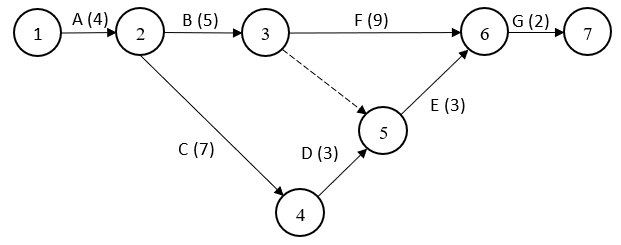
\includegraphics[width=0.5\paperwidth]{C:/Users/Admin/Desktop/Github/question_bank/LyX/static/img/9597-RVHS-2019-P2-Q3-1}
\par\end{center}

\noindent \begin{center}
\begin{tabular}{|c|c|c|}
\hline 
\textbf{Activity} & \textbf{Description} & \textbf{Duration (week)}\tabularnewline
\hline 
A & Specification & 4\tabularnewline
\hline 
B & Installation of datastore servers & 5\tabularnewline
\hline 
C & Development & 7\tabularnewline
\hline 
D & Unit Testing & 3\tabularnewline
\hline 
E & System testing & 3\tabularnewline
\hline 
F & Conversion of existing data files to new format & 9\tabularnewline
\hline 
G & UAT & 2\tabularnewline
\hline 
\end{tabular}
\par\end{center}
\begin{enumerate}
\item Explain the significance of the dotted line. \hfill{}{[}1{]}
\item Draw a Gantt chart based on the above information.\hfill{} {[}3{]}
\item State the impact on the project if activity F duration is cut by 3
weeks.\hfill{} {[}2{]}
\item State the purpose of the project proposal.\hfill{} {[}1{]}
\item State 2 important topics in the project proposal. \hfill{}{[}1{]}
\end{enumerate}